\documentclass{article}
\usepackage{graphicx,amsmath}
\begin{document}
\title{Further explanation of discontinuities in time evolution in finf}
\author{Steven Dorsher}
\maketitle

\section{Higher resolution in time at perihelion and aphelion}

Higher resolution in time at perihelion and aphelion reveals some narrower spikes, while some remain the same widht, as well as features in other modes. This cannot be explained by only resolution issues due to mode spatial resolution or else it would be primarily present at aphelion and higher mode, and that is not the case. It is possible that aphelion and perihelion, and that high mode and low mode features are two different phenomena.

Here is a list of bad modes: 2,3,4,5,26,27,28,29,30

\begin{figure}
  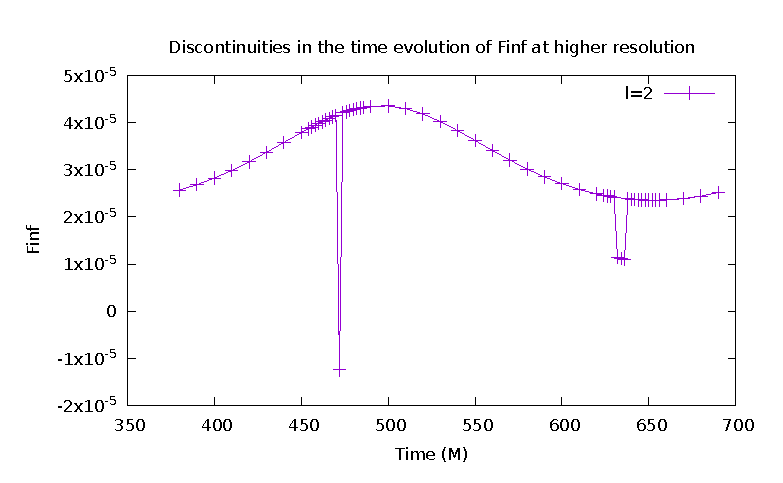
\includegraphics{FinfTimel2}
\end{figure}
\begin{figure}
  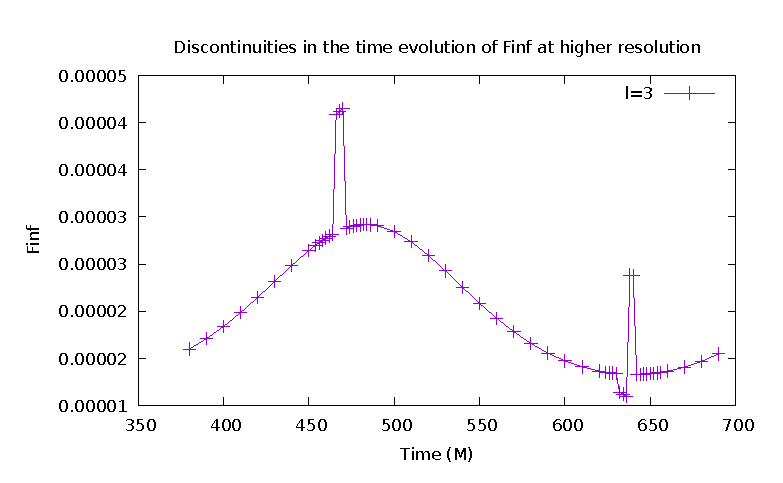
\includegraphics{FinfTimel3}
\end{figure}
\begin{figure}
  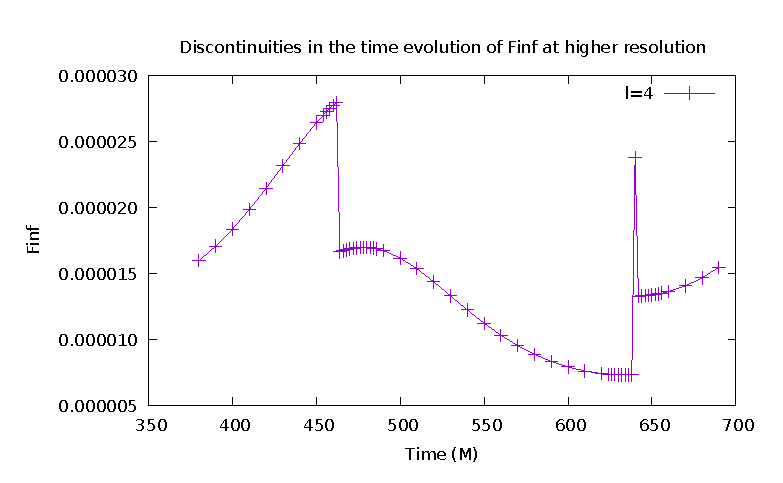
\includegraphics{FinfTimel4}
\end{figure}
\begin{figure}
  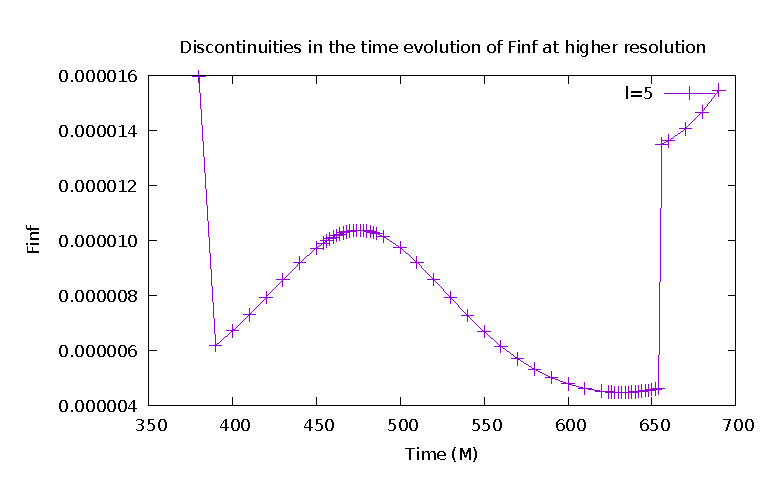
\includegraphics{FinfTimel5}
\end{figure}
\begin{figure}
  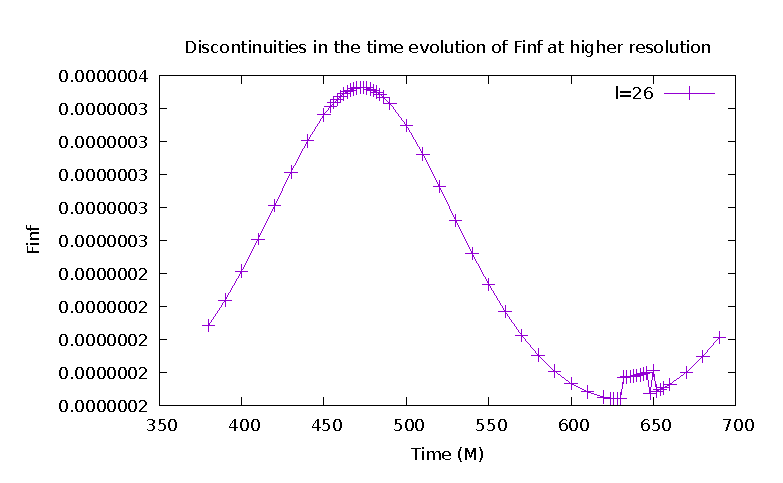
\includegraphics{FinfTimel26}
\end{figure}
\begin{figure}
  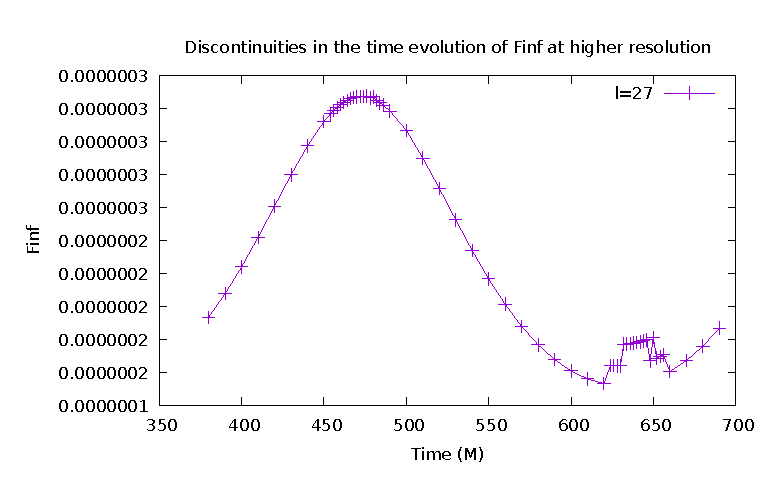
\includegraphics{FinfTimel27}
\end{figure}
\begin{figure}
  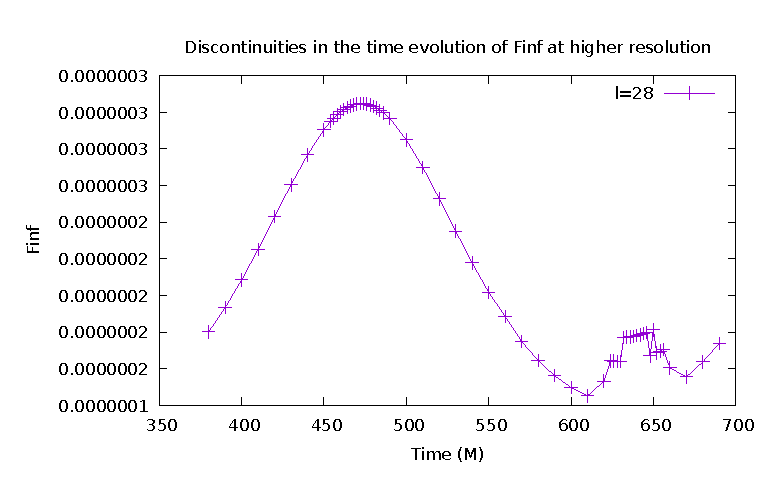
\includegraphics{FinfTimel28}
\end{figure}
\begin{figure}
  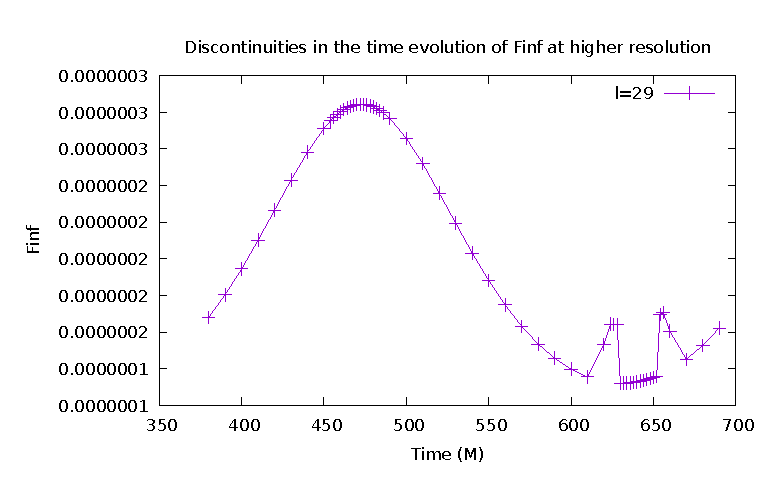
\includegraphics{FinfTimel29}
\end{figure}
\begin{figure}
  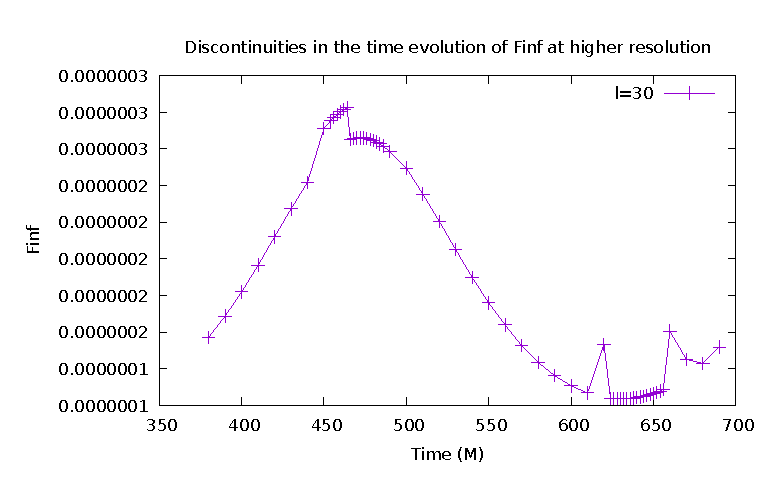
\includegraphics{FinfTimel30}
\end{figure}



\section{Examining plots of the best finf method}


I plotted the starting DG order determined by chosing the highest DG order that did not produce a NaN. This is on the theory that they all looked like Mode 6, which they seemed to for many other times. I have not double checked that. However,this theory does seem to produce smooth time evolution curves for many modes for many times. Here are many plots. If a mode is excluded, it is because it looked like the mode or several modes before it. These are for time 470 M, which was bad in mode 3 (though I might have confused mode 3 and mode 2). These modes are numbered from zero.

\begin{figure}
  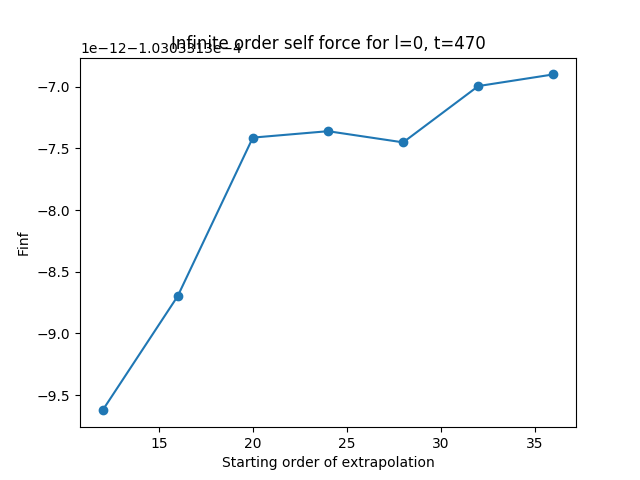
\includegraphics{bestfinfselectorplott470l0}
\end{figure}
\begin{figure}
  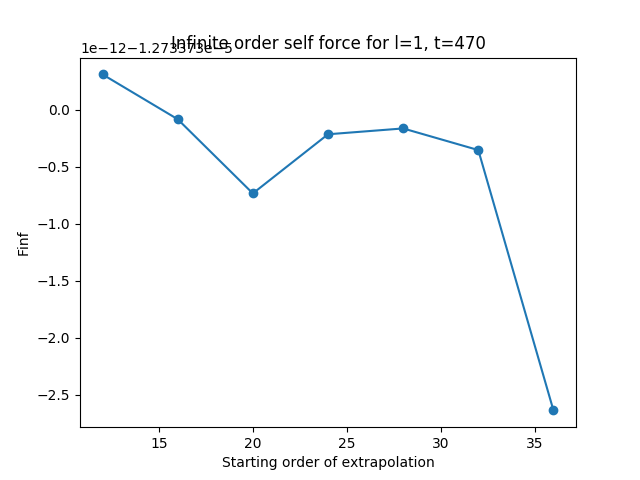
\includegraphics{bestfinfselectorplott470l1}
\end{figure}
\begin{figure}
  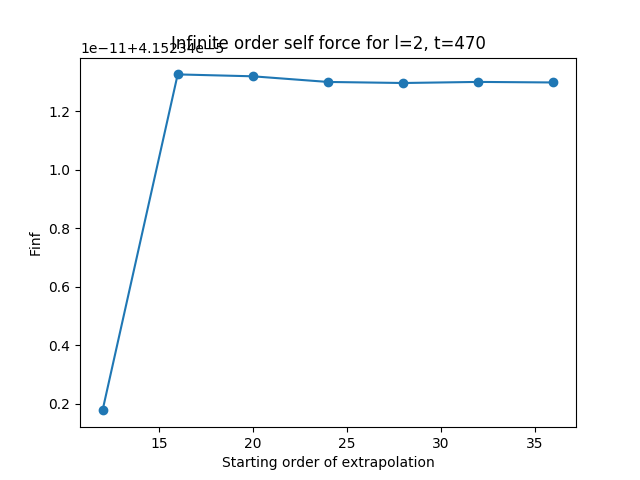
\includegraphics{bestfinfselectorplott470l2}
\end{figure}
\begin{figure}
  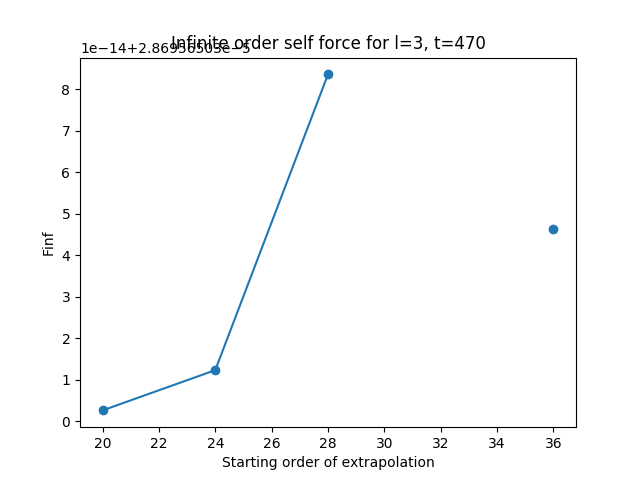
\includegraphics{bestfinfselectorplott470l3}
\end{figure}
\begin{figure}
  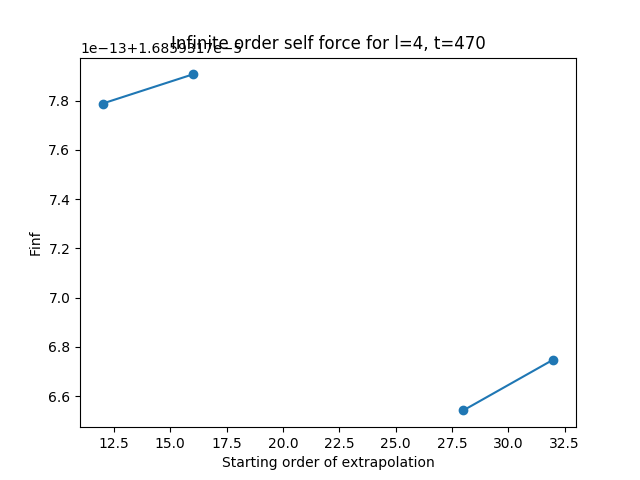
\includegraphics{bestfinfselectorplott470l4}
\end{figure}
\begin{figure}
  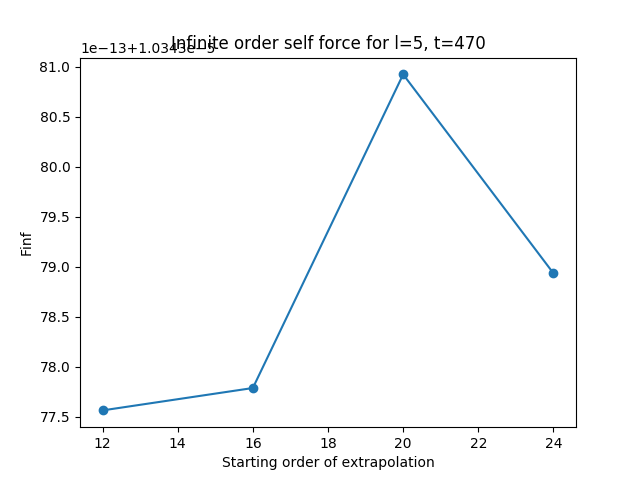
\includegraphics{bestfinfselectorplott470l5}
\end{figure}
\begin{figure}
  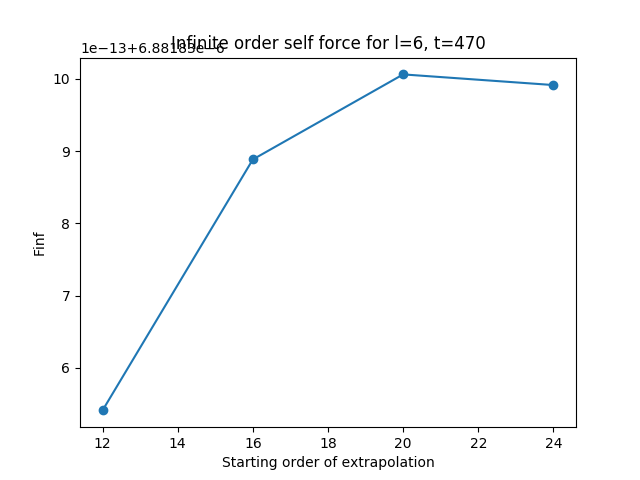
\includegraphics{bestfinfselectorplott470l6}
\end{figure}
\begin{figure}
  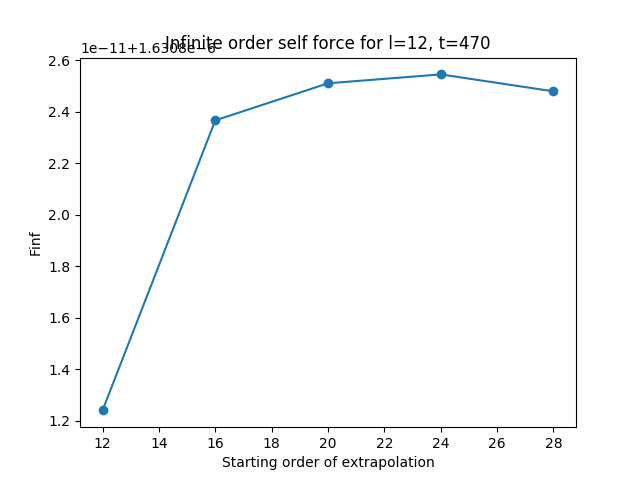
\includegraphics{bestfinfselectorplott470l12}
\end{figure}
\begin{figure}
  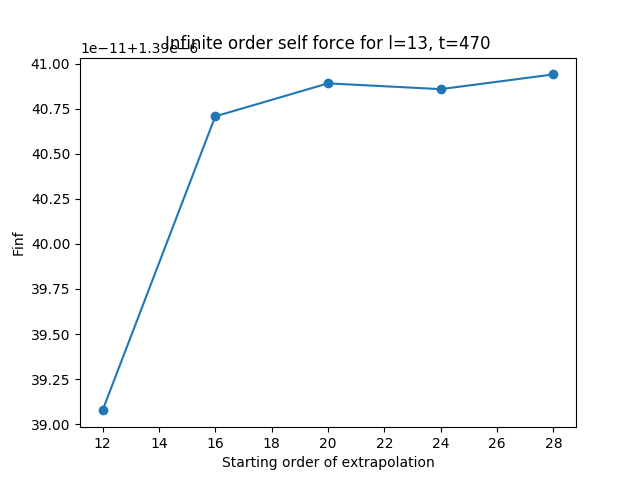
\includegraphics{bestfinfselectorplott470l13}
\end{figure}
\begin{figure}
  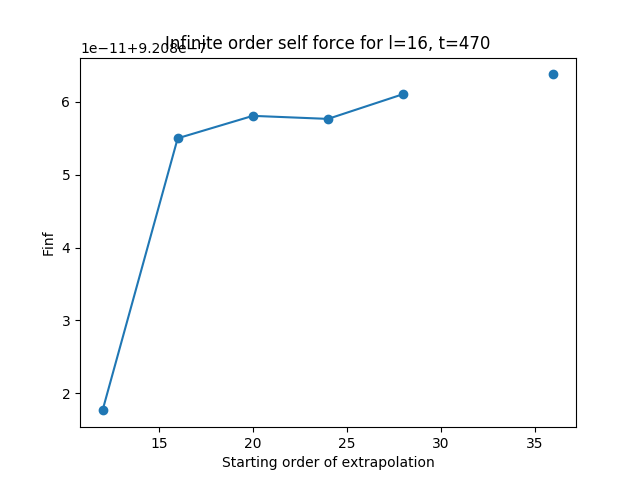
\includegraphics{bestfinfselectorplott470l16}
\end{figure}
\begin{figure}
  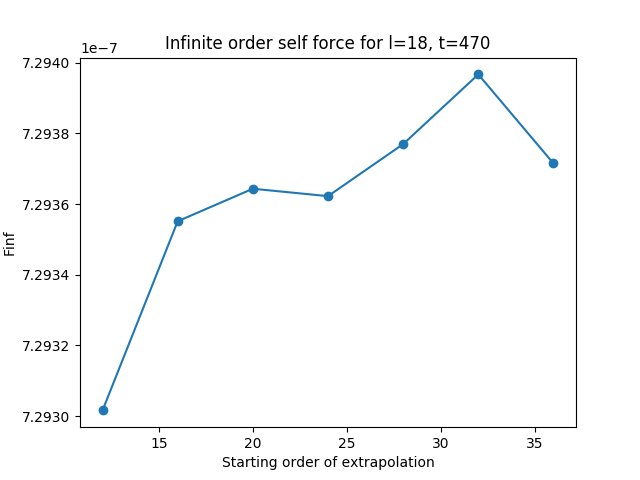
\includegraphics{bestfinfselectorplott470l18}
\end{figure}
\begin{figure}
  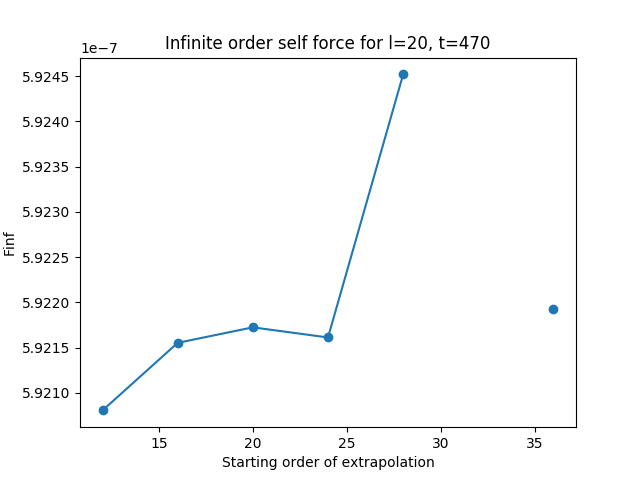
\includegraphics{bestfinfselectorplott470l20}
\end{figure}
\begin{figure}
  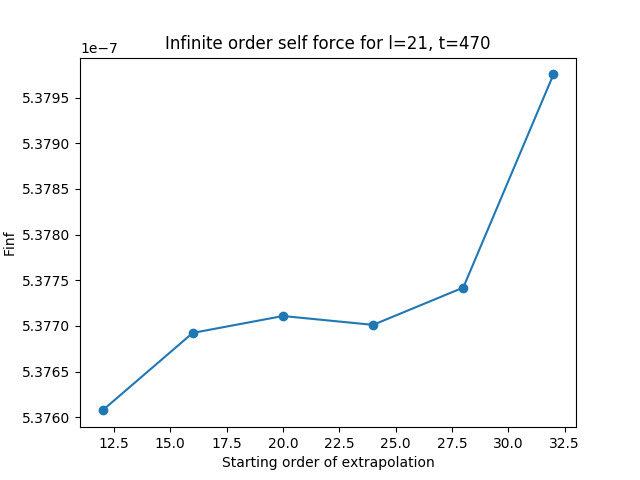
\includegraphics{bestfinfselectorplott470l21}
\end{figure}
\begin{figure}
  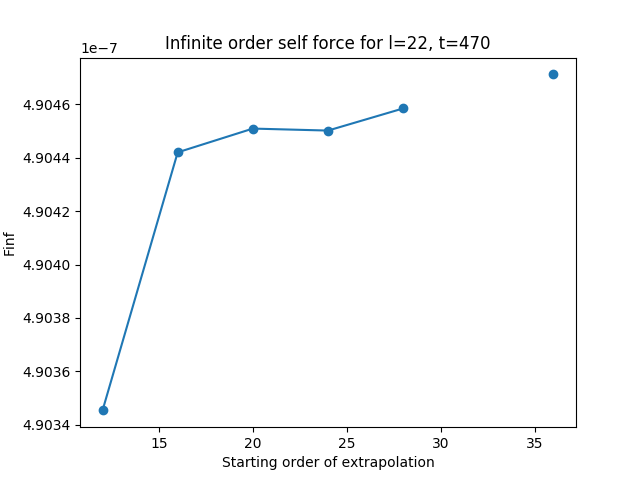
\includegraphics{bestfinfselectorplott470l22}
\end{figure}
\begin{figure}
  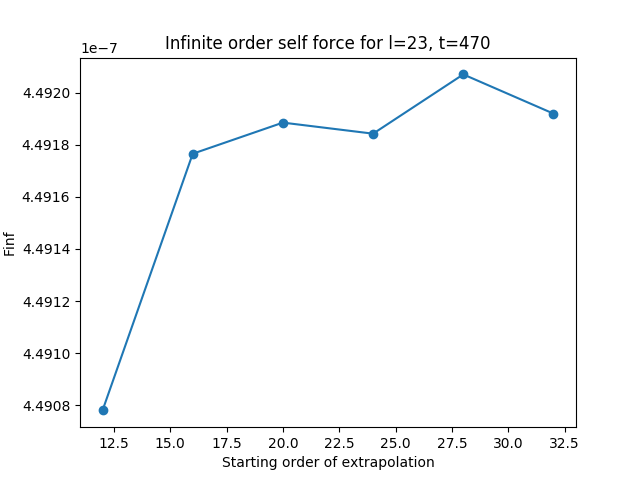
\includegraphics{bestfinfselectorplott470l23}
\end{figure}
\begin{figure}
  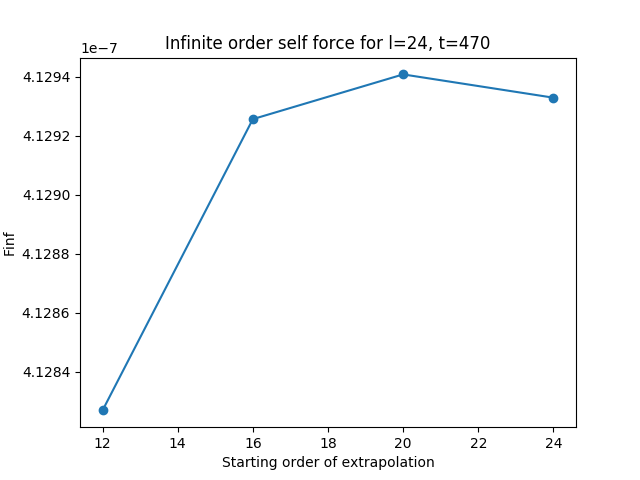
\includegraphics{bestfinfselectorplott470l24}
\end{figure}
\begin{figure}
  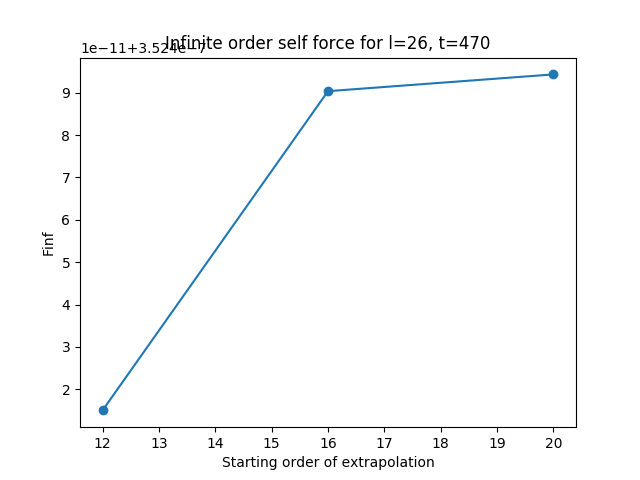
\includegraphics{bestfinfselectorplott470l26}
\end{figure}
\begin{figure}
  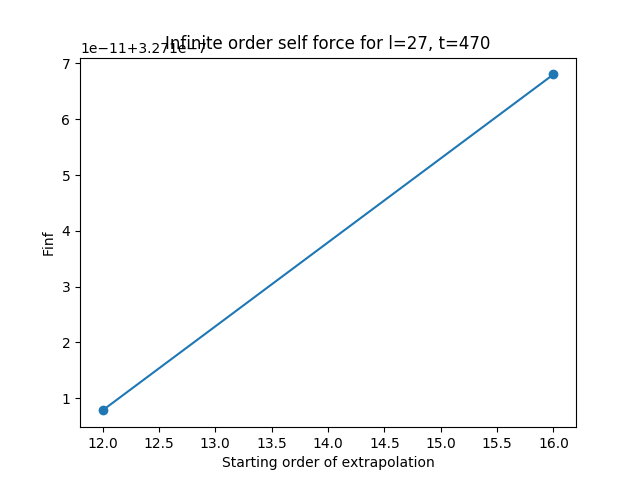
\includegraphics{bestfinfselectorplott470l27}
\end{figure}
\begin{figure}
  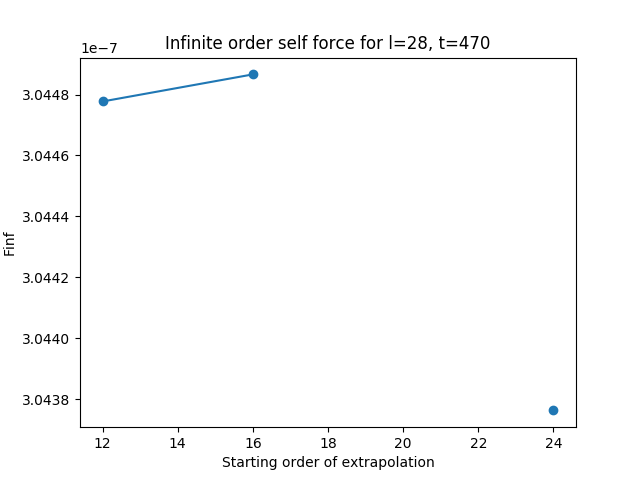
\includegraphics{bestfinfselectorplott470l28}
\end{figure}
\begin{figure}
  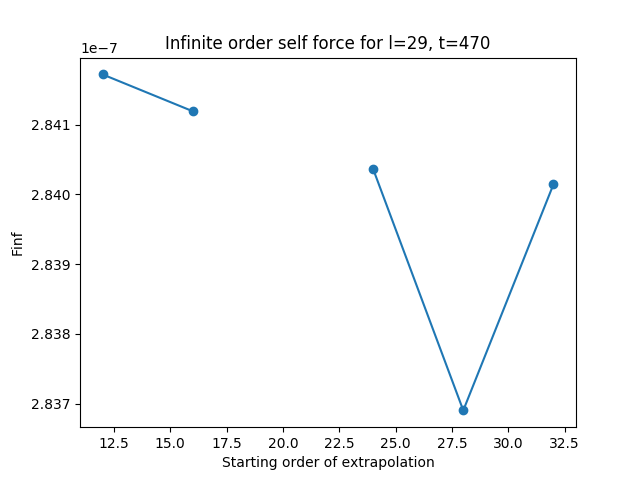
\includegraphics{bestfinfselectorplott470l29}
\end{figure}
\begin{figure}
  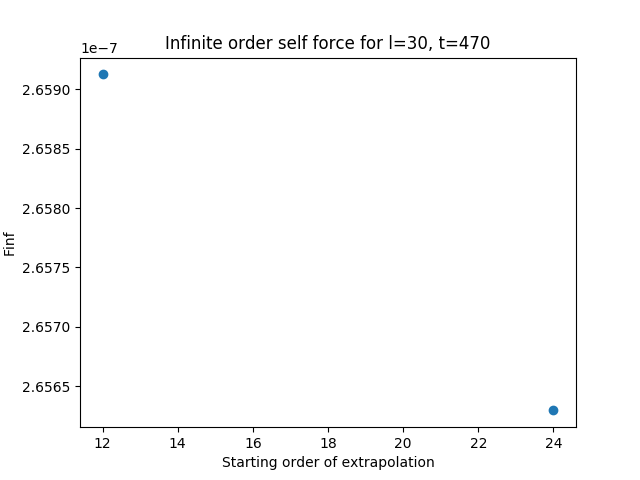
\includegraphics{bestfinfselectorplott470l30}
\end{figure}



\section{Checking the exponential convergence of a couple of the bad modes}

I checked modes three and four by subtracting the offsets using subtractoffset.py, an automated routine to subtract the offset. I attempted to get closer to eliminating roundoff using plotconvergence.py, a routine that allows manual adjustment of finf; however, something is wrong with the xaxis scaling in this routine and it seems to be stuck in loglog scale. I also can't get the y axis to display a scale. I should try Mathematica tomorrow.

Here are the four plots I generated. Using nmaxFinfOverTime\_finf\_highrez.csv and the corresponding nmax file, I determined the starting order indices that corresponded to the time of 470 and the mode l=3 or l=4. They were 6 and 1. I then entered the mode number, time and i1 into subtractoffset and obtained the plots shown below. One of the plots for l=4 is for i=3 instead of i=1 because it gave a closer, but still bad, result. It is clear that something further still needs to be subtracted before roundoff error is reached.


\begin{figure}
  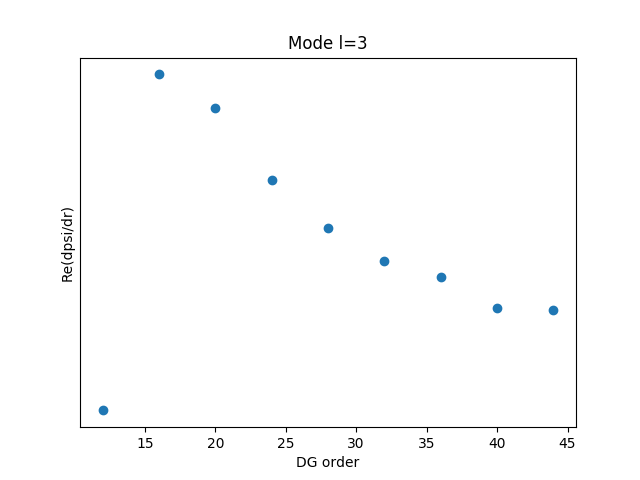
\includegraphics{subtractoffsett470l3}
  \caption{l=3,i=6,t=470, what was selected by the best finf finder}
\end{figure}
\begin{figure}
  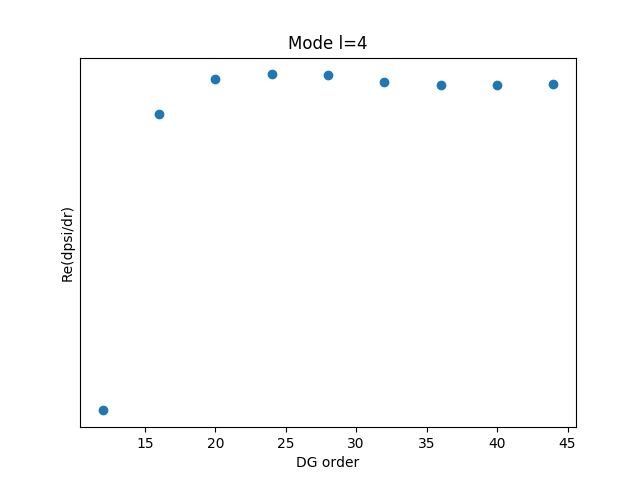
\includegraphics{subtractoffsett470l4i1}
  \caption{l=4,i=1,t=470, what was selected by the best finf finder}
\end{figure}

\begin{figure}
  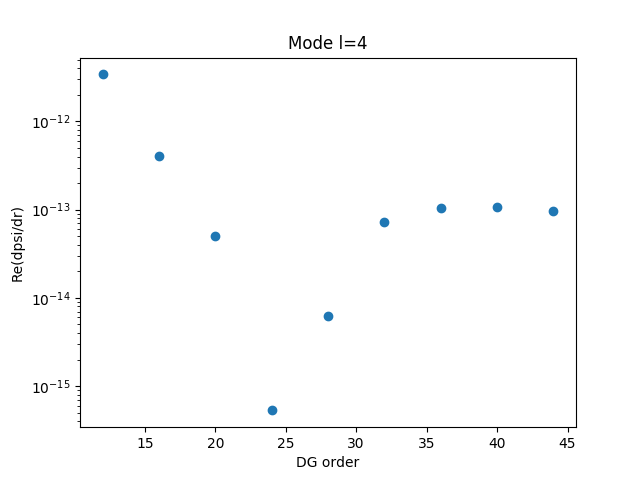
\includegraphics{subtractoffsett470l4i3}
  \caption{l=4,i=3,t=470, obviously ``better'' than the ``best'' finf}
\end{figure}
    

\section{To Do}

\begin{itemize}
\item Finish checking the exponential convergence of the bad
  modes. Both in terms of doing better subtractions by hand (in
  Mathematica?) and in terms of checking all the bad modes and some of
  the good modes for comparison.
\item Find a better means of determining the ``Best'' order to start with, if fixing the exponential convergence does not fix those plots.
\item Double check the starting DG order versus finf plot for other better times.

  \item double check the distinction between mode three and mode 2 in any analysis where it matters. I think the bad times are similar enough where it should be okay. 

\end{itemize}


\end{document}
